%%%%%%%%%%%%%%%%%%%%%%%%%%%%%%%%%%%%%%%%%
% Thin Sectioned Essay
% LaTeX Template
% Version 1.0 (3/8/13)
%
% This template has been downloaded from:
% http://www.LaTeXTemplates.com
%
% Original Author:
% Nicolas Diaz (nsdiaz@uc.cl) with extensive modifications by:
% Vel (vel@latextemplates.com)
%
% License:
% CC BY-NC-SA 3.0 (http://creativecommons.org/licenses/by-nc-sa/3.0/)
%
%%%%%%%%%%%%%%%%%%%%%%%%%%%%%%%%%%%%%%%%%

%----------------------------------------------------------------------------------------
%	PACKAGES AND OTHER DOCUMENT CONFIGURATIONS
%----------------------------------------------------------------------------------------

\documentclass[a4paper, 12pt]{article} % Font size (can be 10pt, 11pt or 12pt) and paper size (remove a4paper for US letter paper)

\usepackage[protrusion=true,expansion=true]{microtype} % Better typography
\usepackage{graphicx} % Required for including pictures
\usepackage[utf8]{inputenc}
\usepackage[margin=1.0in]{geometry}
\usepackage{url}
\usepackage{fancyhdr}
\usepackage{amsmath}
\usepackage{setspace}
\usepackage{enumitem}
\usepackage{float}
\setlength\parindent{0pt} % Removes all indentation from paragraphs

\usepackage[T1]{fontenc} % Required for accented characters
\usepackage{times} % Use the Palatino font

\usepackage{listings}
\usepackage{color}
\lstset{mathescape}

\definecolor{dkgreen}{rgb}{0,0.6,0}
\definecolor{gray}{rgb}{0.5,0.5,0.5}
\definecolor{mauve}{rgb}{0.58,0,0.82}

\lstset{frame=tb,
   language=c++,
   aboveskip=3mm,
   belowskip=3mm,
   showstringspaces=false,
   columns=flexible,
   basicstyle={\small\ttfamily},
   numbers=none,
   numberstyle=\tiny\color{gray},
   keywordstyle=\color{blue},
   commentstyle=\color{dkgreen},
   stringstyle=\color{mauve},
   breaklines=true,
   breakatwhitespace=true
   tabsize=3
}
\linespread{1.00} % Change line spacing here, Palatino benefits from a slight increase by default

\makeatletter
\renewcommand{\@listI}{\itemsep=0pt} % Reduce the space between items in the itemize and enumerate environments and the bibliography

\renewcommand\abstractname{Résumé}
\renewcommand\refname{Références}
\renewcommand\contentsname{Table des matières}
\renewcommand{\maketitle}{ % Customize the title - do not edit title and author name here, see the TITLE block below
\begin{center} % Right align

\vspace*{25pt} % Some vertical space between the title and author name
{\LARGE\@title} % Increase the font size of the title

\vspace{125pt} % Some vertical space between the title and author name

{\large\@author} % Author name

\vspace{125pt} % Some vertical space between the author block and abstract
Dans le cadre du cours
\\INF4705 - Analyse et conception d'algorithmes
\vspace{125pt} % Some vertical space between the author block and abstract
\\\@date % Date
\vspace{125pt} % Some vertical space between the author block and abstract

\end{center}
}

%----------------------------------------------------------------------------------------
%	TITLE
%----------------------------------------------------------------------------------------

\title{TP2} 

\author{\textsc{Guillaume Arruda 1635805\\Raphael Lapierre 1644671} % Author
\vspace{10pt}
\\{\textit{École polytechnique de Montréal}}} % Institution

\date{18 mars 2016} % Date

%----------------------------------------------------------------------------------------

\begin{document}

\thispagestyle{empty}
\clearpage\maketitle % Print the title section
\pagebreak[4]
%\tableofcontents
%\pagebreak[4]
%----------------------------------------------------------------------------------------
%	En tête et pieds de page 
%----------------------------------------------------------------------------------------

\setlength{\headheight}{15.0pt}
\pagestyle{fancy}
\fancyhead[L]{INF4705}
\fancyhead[C]{}
\fancyhead[R]{TP2}
\fancyfoot[C]{\textbf{page \thepage}}

%----------------------------------------------------------------------------------------
%	ESSAY BODY
%----------------------------------------------------------------------------------------
\section*{Introduction}
Le but de ce laboratoire était d'implémenter et d'analyser différents algorithmes pour la mise en place de succursale de la chaine
W\&A. 3 algorithmes d'optimisations de solutions ont été créés pour maximiser les profits tout en respectant les contraintes de production
locales. Au niveau académique, ce laboratoire nous a permis de pratiquer l'implémentation d'algorithmes pour des problèmes réelles simplifiés. Les algorithmes implémentés sont: vorace probabiliste, à heuristique d'amélioration locale et à programmation dynamique.
\section*{Jeu de données}
Les jeux de données utilisé pour tester nos algorithmes sont composés de plusieurs locations qui possèdent un numéro d'identification, un revenu et une consommation de poulet. Chaque jeu de données possède aussi une production de poulet maximale qui correspond à la contrainte pour nos algorithmes. Le nombre de location testé varie de 10 à 1000 et la consommation maximale de 11 à 49097.
\section*{Présentation des résultats}
\begin{table}[H]
\caption{Temps moyen d'exécution de l'algorithme vorace}
\centering
\begin{tabular}{| l | c | c | r |}
\hline
taille d'échantillon & production moyenne & temps moyen(ms)  & Revenu moyen(\$)\\
\hline
10 & 11 & 0.0414 & 11.78\\
\hline
10 & 101 & 0.0395 & 104.2\\
\hline
10 & 1001 & 0.0445 & 1101.875\\
\hline
20 & 11 & 0.0529 & 12.2\\
\hline
20 & 101 & 0.0536 & 114.8\\
\hline
20 & 1001 & 0.0545 & 1148.33\\
\hline
50 & 11 & 0.0934 & 19.1\\
\hline
50 & 101 & 0.0986 & 180.3\\
\hline
50 & 1001 & 0.093 & 1761.9\\
\hline
100 & 28.375 & 0.244 & 35.78\\
\hline
100 & 282.625 & 0.238 & 343.88\\
\hline
100 & 2255 & 0.243 & 3152.9\\
\hline
200 & 48.375 & 0.787 & 64.8\\
\hline
200 & 462 & 0.833 & 616.6.78\\
\hline
200 & 5240 & 0.809 & 6317.78\\
\hline
500 & 150.2 & 4.80 & 160.9\\
\hline
500 & 1388.2 & 4.89  & 1504.2\\
\hline
500 & 13367.2 & 5.31 & 14452.1\\
\hline
1000 & 302 & 18.83 & 321\\
\hline
1000 & 2780 & 19.33 & 2946.6\\
\hline
1000 & 27102.9 & 19.26 & 28935.2\\
\hline
\end{tabular}
\end{table}
\begin{table}[H]
\caption{Temps moyen d'exécution de l'algorithme d'heuristique d'amélioration locale}
\centering
\begin{tabular}{| l | c | c | r |}
\hline
taille d'échantillon & production moyenne & temps moyen(ms)  & Revenu moyen\\
\hline
10 & 11 & 0.0041 & 12\\
\hline
10 & 101 & 0.04 & 105.2\\
\hline
10 & 1001 & .256 & 1106.125\\
\hline
20 & 11 & 0.0061 & 12.7\\
\hline
20 & 101 & 0.0516 & 117.8\\
\hline
20 & 1001 & 0.0517 & 1230.44\\
\hline
50 & 11 & 0.747 & 21.2\\
\hline
50 & 101 & 0.247 & 200.6\\
\hline
50 & 1001 & 0.173 & 1961.5\\
\hline
100 & 28.375 & 2.32 & 42.22\\
\hline
100 & 282.625 & 2.13 & 401.56\\
\hline
100 & 2255 & 1.65 & 3673.7\\
\hline
200 & 48.375 & 47.28 & 82\\
\hline
200 & 462 & 55.60 & 737.9\\
\hline
200 & 5240 & 68.49 & 7603.33\\
\hline
500 & 150.2 & 5224.5 & 206.5\\
\hline
500 & 1388.2 & 6626.6 & 1855.9\\
\hline
500 & 13367.2 & 7358.7 & 18018.5\\
\hline
1000 & 302 & 158667.9 & 416.4\\
\hline
1000 & 2780 & 210166.5 & 3721.7\\
\hline
1000 & 27102.9 & 231598.5 & 36458.6\\
\hline
\end{tabular}
\end{table}
\begin{table}[H]
\caption{Temps moyen d'exécution de l'algorithme de programmation dynamique}
\centering
\begin{tabular}{| l | c | c | r |}
\hline
taille d'échantillon & production moyenne & temps moyen(ms)  & Revenu moyen(\$)\\
\hline
10 & 11 & 0.000494 & 13.11\\
\hline
10 & 101 & 0.0086 & 108.2\\
\hline
10 & 1001 & 0.049 & 1106.125\\
\hline
20 & 11 & 0.0037 & 13.9\\
\hline
20 & 101 & 0.0131 & 119.9\\
\hline
20 & 1001 & 0.104 & 1235.56\\
\hline
50 & 11 & 0.0061 & 22.6\\
\hline
50 & 101 & 0.042 & 203.6\\
\hline
50 & 1001 & 0.0370 & 1967.6\\
\hline
100 & 28.375 & 0.0196 & 43.33\\
\hline
100 & 282.625 & 0.166 & 403.67\\
\hline
100 & 2255 & 1.49 & 3675.7\\
\hline
200 & 48.375 & 0.0676 & 83.8\\
\hline
200 & 462 & 0.581 & 741\\
\hline
200 & 5240 & 6.29 & 7610.78\\
\hline
500 & 150.2 & 0.388 & 209.5\\
\hline
500 & 1388.2 & 3.72 & 1858.8\\
\hline
500 & 13367.2 & 37.2 & 18027.2\\
\hline
1000 & 302 & 1.610 & 421\\
\hline
1000 & 2780 & 15.39 & 3724\\
\hline
1000 & 27102.9 & 188.30 & 36469.1\\
\hline
\end{tabular}
\end{table}
\section*{Analyse et discussion}
\subsection*{Algorithme vorace probabiliste}
\subsubsection*{Analyse asymptotique}
\subsubsection*{Analyse hybride}
L'analyse hybride de l'algorithme vorace probabiliste a été effectué avec le test de puissance.
\begin{figure}[H]
    \centering
    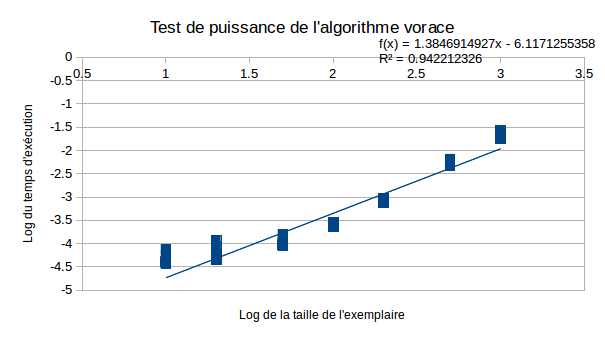
\includegraphics[width=0.95\textwidth]{Figure/AlgorithmeVorace}
\end{figure}

\subsection*{Algorithme heuristique d'amélioration locale}
\subsubsection*{Analyse asymptotique}
\subsubsection*{Analyse hybride}

\subsection*{Algorithme de programmation dynamique}
\subsubsection*{Analyse asymptotique}
    L'algorithme implémenté pour cette section est assez simple à analyse de façon
    asymptotique. Un tableau de taille $i\times j$ doit être rempli pour avoir une solution.
    Dans notre cas, $i$ représente le nombre de locations différentes et $j$ représente la quantité
    totale de poulet pouvant être acheté du fournisseur. Remplir ce tableau nécéssite de passer une seule
    fois sur chacune des cases. On a donc, $\Theta(ij)$. Ensuite, pour obtenir la solution, on doit 
    revenir de la case finale du tableau vers la case initiale. En pire cas cette marche peut prendre
    $ij$ opérations. Cela n'a donc pas d'effet sur la complexité algorithmique. Bref, il est possible 
    d'affirmer que cet algorithme est élément de $\Theta(ij)$.
\subsubsection*{Analyse hybride}
    Dans le cas de l'analyse hybride, le test de puissance a été effectué. Pour se faire,
    nous avons tracé un graphique en trois dimensions des résultats et trouvé le plan
    passant par les points qui minimisent l'erreur. Celle-ci est donnée par l'équation

    \begin{equation}
        e = \sum z - ax + by + c
    \end{equation}
    
    où $e$ est l'erreur, $x, y, z$ un trio des points de nos données et a, b, c les constantes du plan
    à optimiser. Nous avons donc trouvé l'équation du plan suivante :

    \begin{equation}
        z = 0.953x + 0.909y - 7.828
    \end{equation}

    En prenant les dérivées partielles par rapport à $x$ et $y$, on trouve : 

    \begin{equation}
        \frac{\partial z}{\partial x} = 0.953
    \end{equation}
    \begin{equation}
        \frac{\partial z}{\partial y} = 0.909
    \end{equation}

    L'équation du test de puissance pour nos données est donnée, quant à elle, par:

    \begin{equation}
        \log f(x,y) = m_{1}\log x + b_{1} + m_{2}\log x + b_{2}
    \end{equation}

    On peut donc déduire, avec $m_{1} = 0.953$ et $m_{2} = 0.909$ que nous avons une complexité
    d'environ $\Theta(x^{0.953}y^{0.909})$ empiriquement ce qui semble bel et bien en accord 
    avec l'analyse théorique de l'algorithme.

    \begin{figure}
    	\centering
        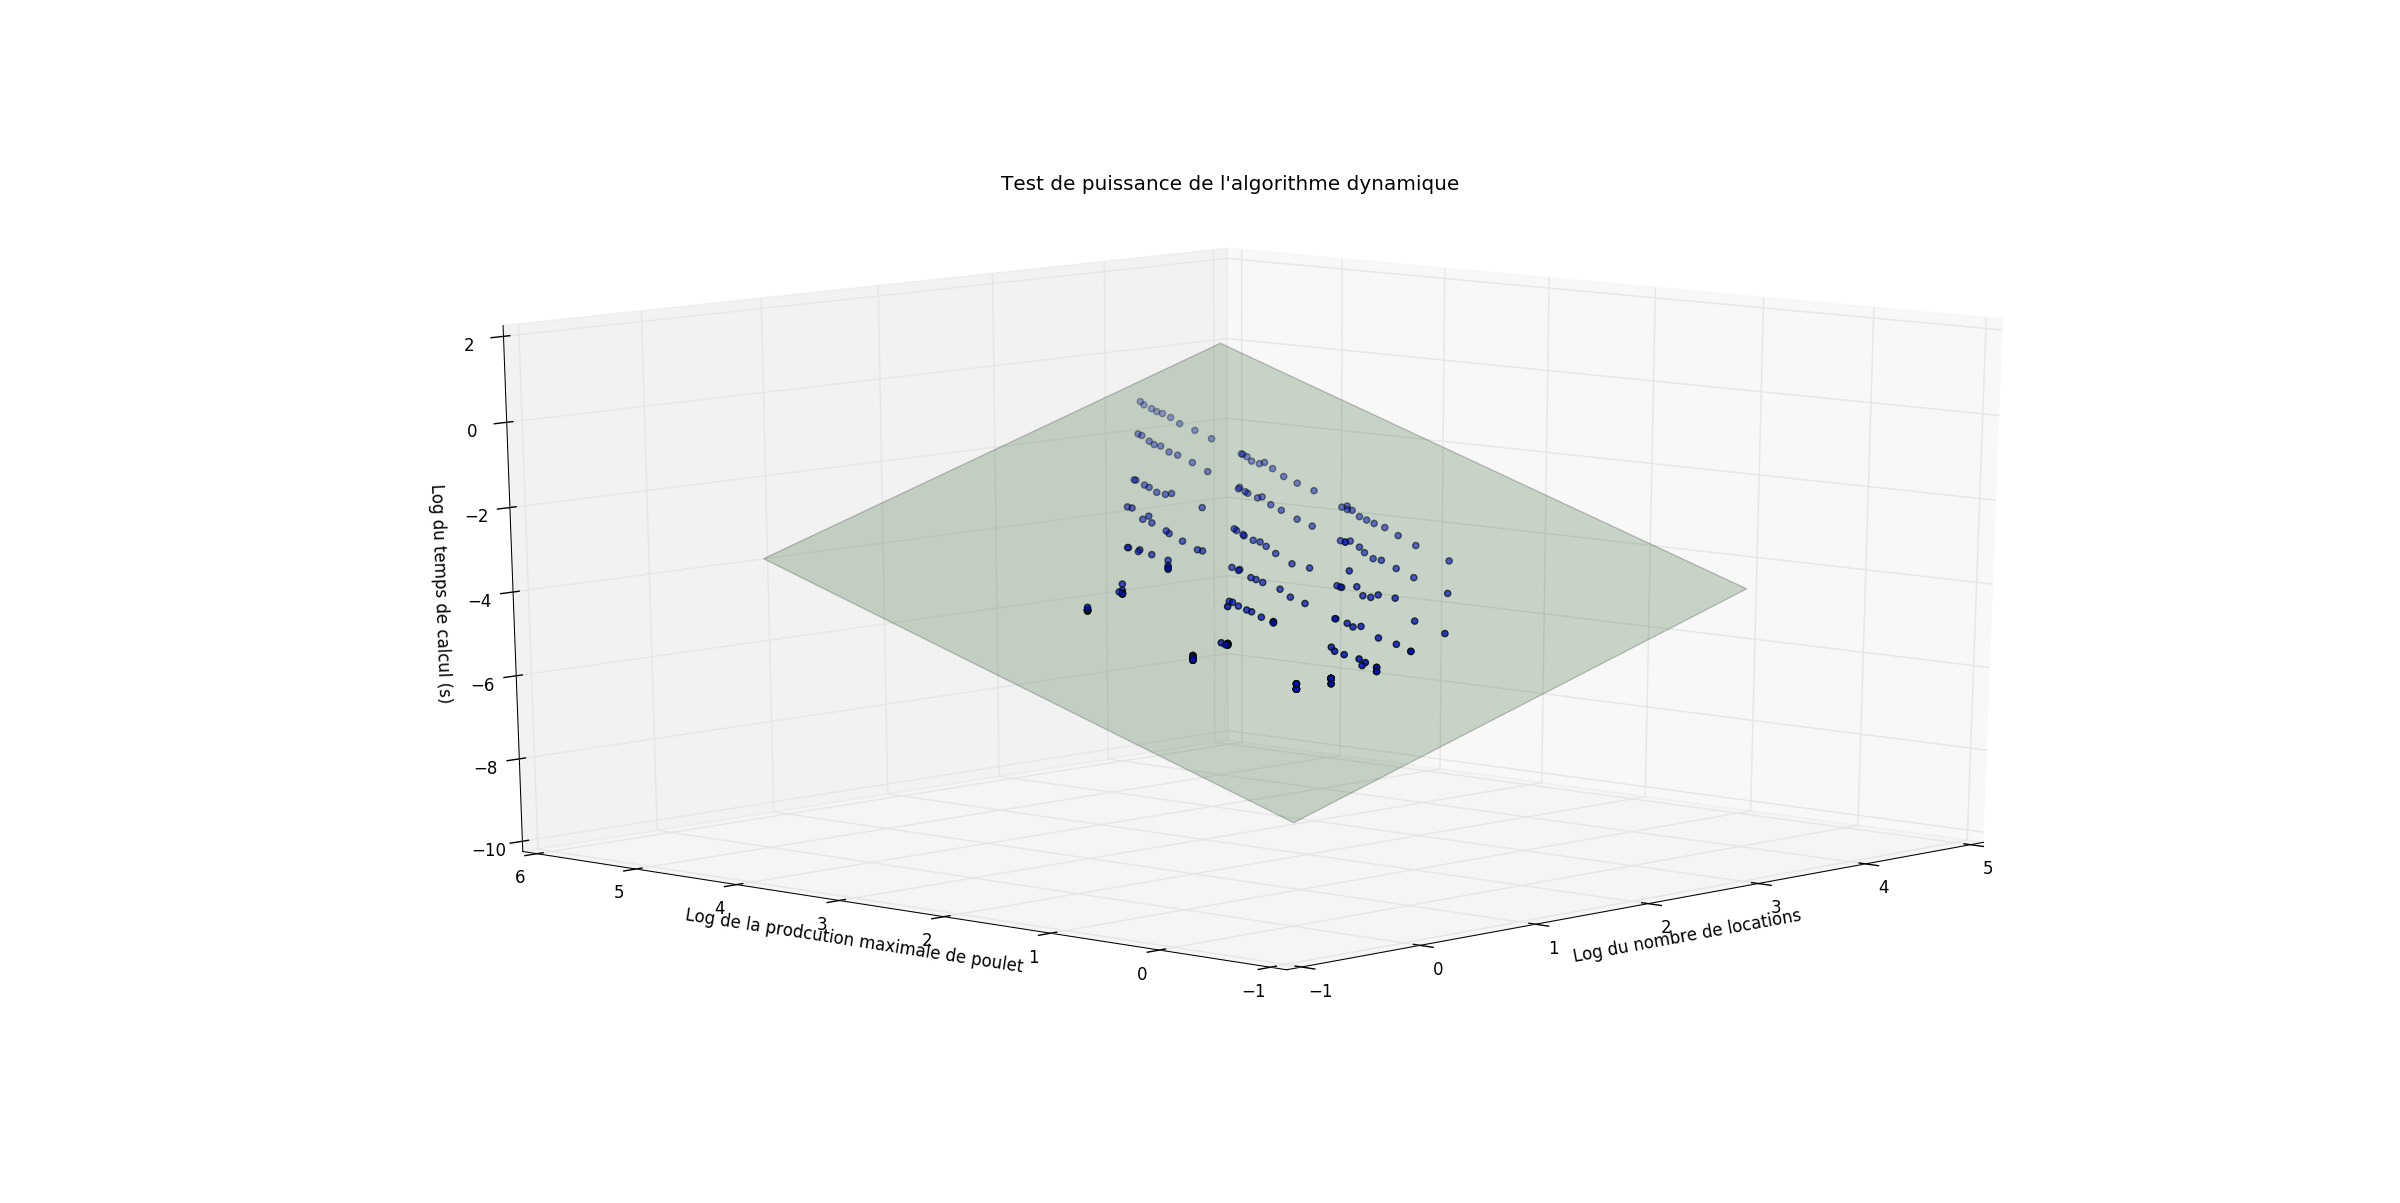
\includegraphics[width=0.95\textwidth]{Figure/AlgorithmeDynamique.png}
    \end{figure}

    \begin{figure}
    	\centering
        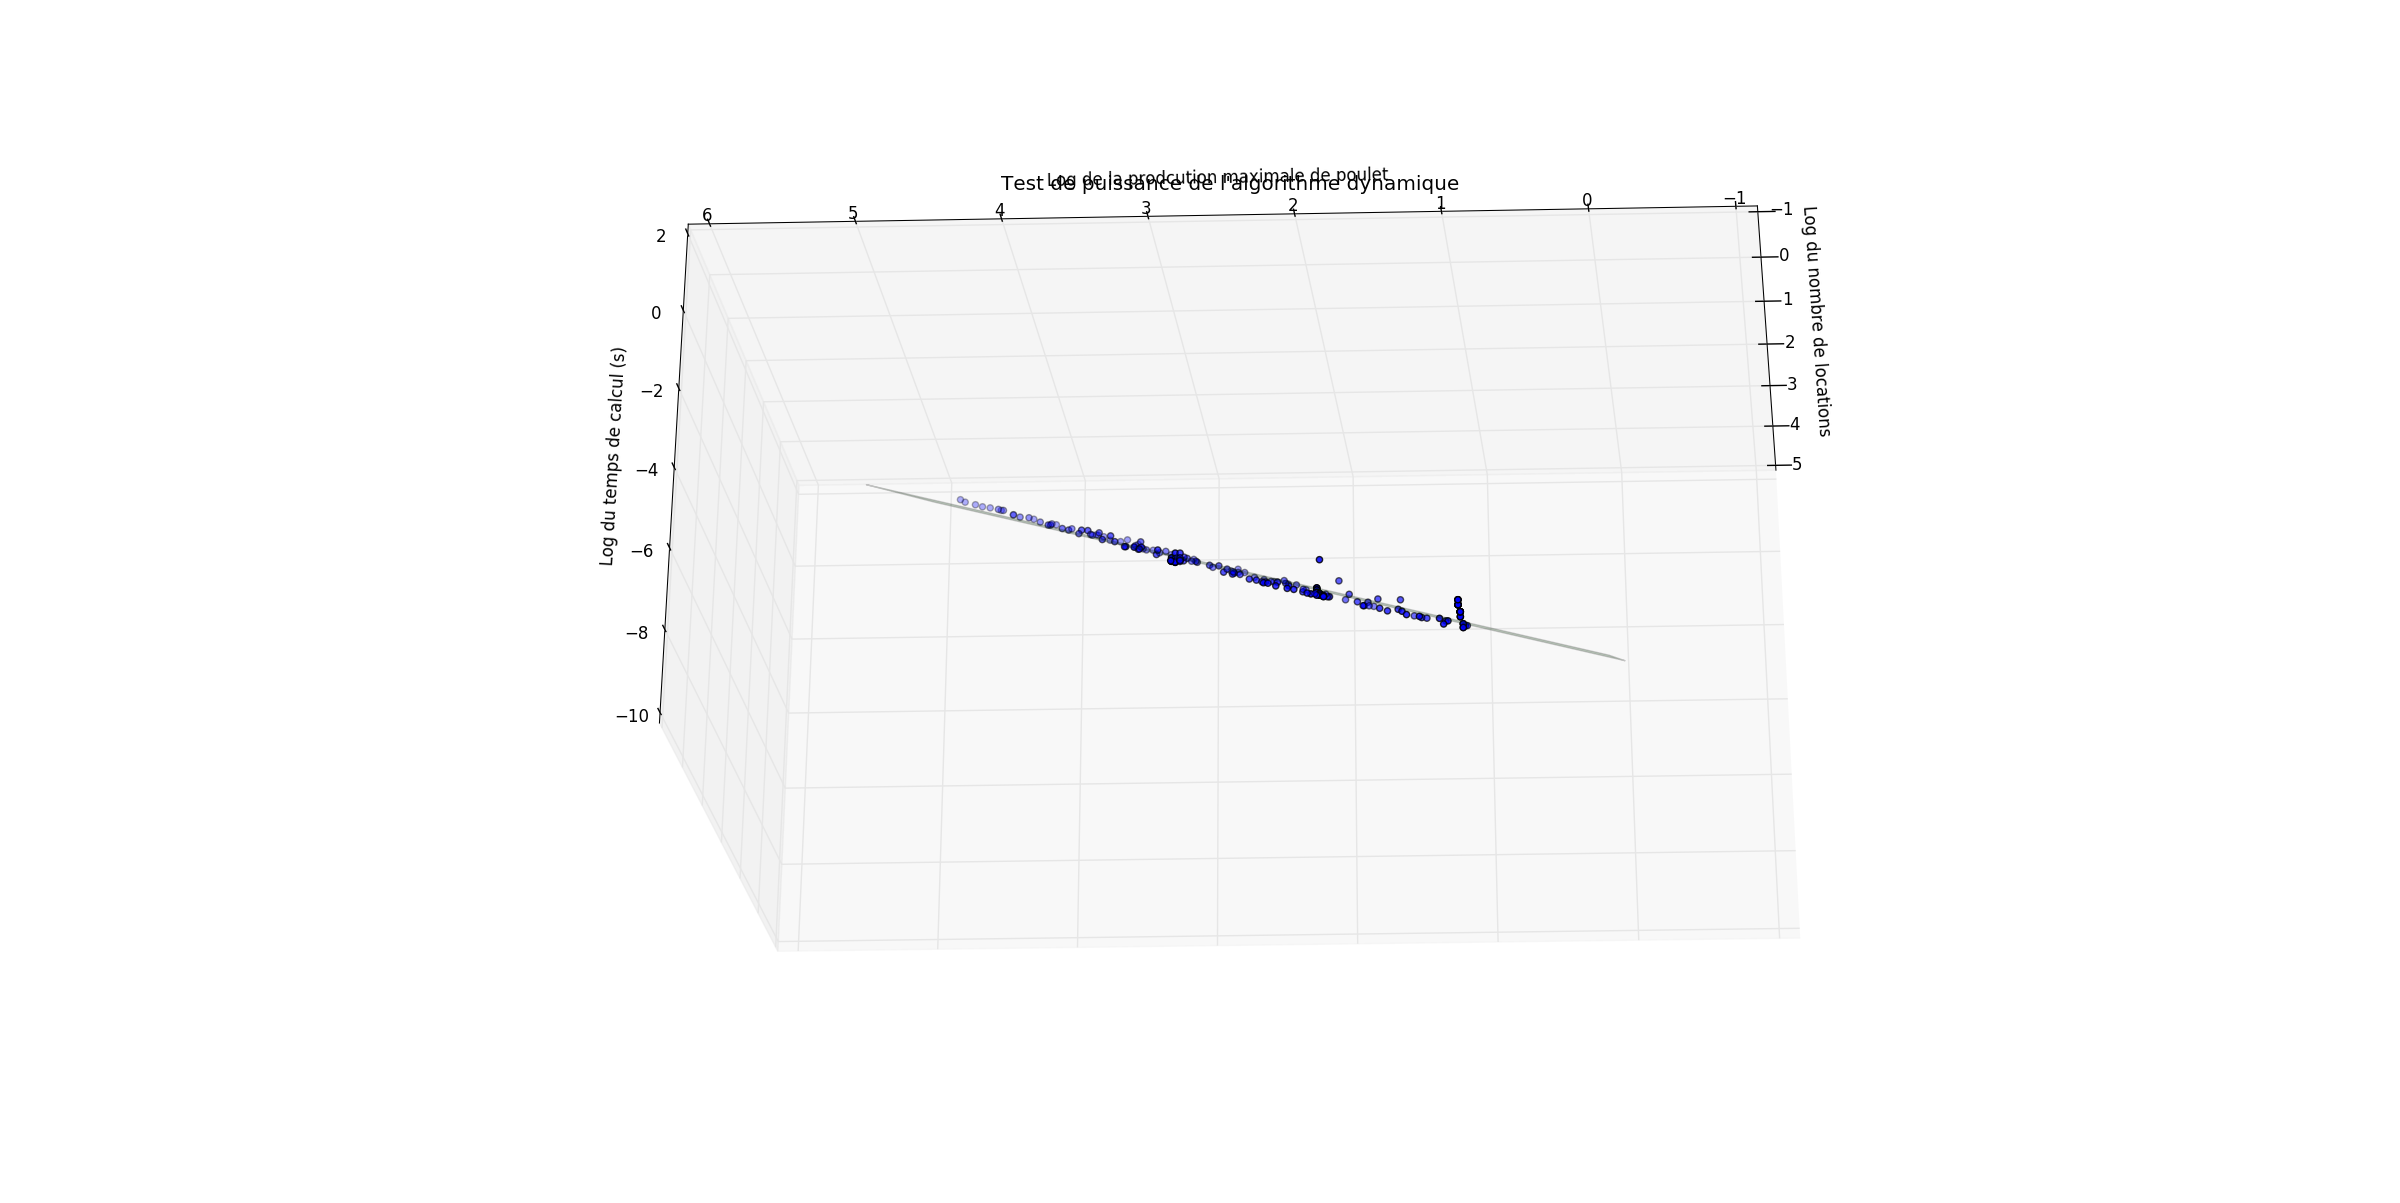
\includegraphics[width=0.95\textwidth]{Figure/AlgorithmeDynamique2.png}
    \end{figure}

    \vspace{12pt}
    En conclusion, cet algorithme est de loin le meilleur selon nos résultats obtenues et le temps
    d'implémentation ainsi que la difficulté ne sont pas supérieur aux autres algorithmes. À la lumière
    des résultats, tant que la quantité de mémoire disponible est suffisante pour effectuer cet algorithme, 
    il est suggéré de l'utiliser.


%----------------------------------------------------------------------------------------
\end{document}
